%-------------------------
%makefile
%(c) H.Buchmann FHNW 2014
%export TEXINPUTS=${HOME}/fhnw/edu/:${HOME}/fhnw/edu/tinL/config/latex:${HOME}/fhnw/edu/config//:
%-------------------------
\documentclass{beamer}
\usepackage{latex/beamer}
%---------------------
%local defines
%(c) H.Buchmann FHNW 2009
%$Id$
%---------------------
\newcommand{\target} {\beaglebone\xspace}
\newcommand{\targetS}{{\bf BBG}\xspace}
\newcommand{\host}   {{\em Host}\xspace}
\newcommand{\targetroot} {{\bf target-root}\xspace}
\newcommand{\kernel} {{\bf kernel}\xspace}
\renewcommand{\c}{{\bf C}\xspace}
\newcommand{\cpp}{{\bf C++}\xspace}
\newcommand{\posix}{{\bf POSIX}\xspace}

\input{/home/buchmann/latex/dirtree/dirtree.tex}

\usepackage[absolute]{textpos}
\setlength{\TPHorizModule}{1mm}
\setlength{\TPVertModule}{1mm}

\begin{document}

\newcommand{\bbb}{{\bf BBB}\xspace}
\newcommand{\uboot}{{U-Boot \xspace}}

\title[Standlone]{Standalone\\Internet of Things}

\frame{\titlepage}

\begin{frame}{Um was geht es ?}{\beaglebone Standalone}
 \begin{itemize}
  \item \bbb startet automatisch
  \item \bbb mit Wi-Fi
  \begin{itemize}
   \item in einem bestehenden Wi-Fi
   \item einem eigenen Wi-Fi
  \end{itemize}
 \end{itemize}
\end{frame}

\begin{frame}{Die Schichten}
\begin{center}
 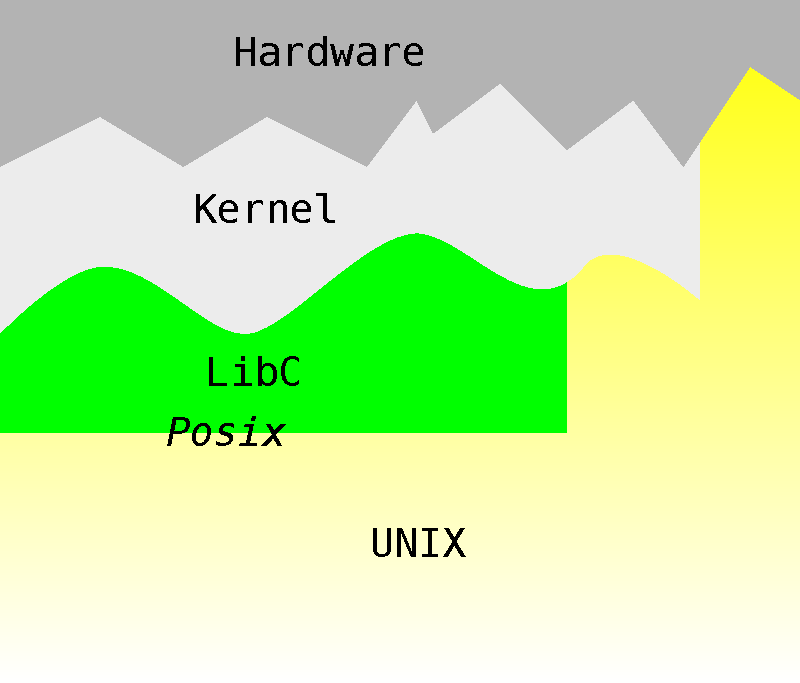
\includegraphics[width=0.75\textwidth]{../../5-kernel/doc/layers.pdf}
\end{center}
\end{frame}

\begin{frame}{Das Ziel}{f�r \bbb}
 \begin{block}{Nach dem Reset:}
 \begin{enumerate}
  \item \uboot startet \kernel
  \item \kernel startet \unix
  \item \unix 
   \begin{itemize}
    \item \cod{/etc/init.d/rcS} 
   \end{itemize}
 \end{enumerate}
 \end{block}
\end{frame}

\begin{frame}{Was wir schon haben}
 \begin{description}[Konfigurationen:]
  \item[Toolchain:] download
  \item[\uboot:] selber gemacht
  \item [\kernel:] selber gemacht
  \item[root Filesystem:] download
  \item[Konfigurationen:]
  \begin{itemize}
   \item \cod{sshd} 
   \item \cod{wpa\_supplicant}
   \item \cod{dhcp}
   \item \cod{route}
   \item \cod{nameserver}
  \end{itemize}
 \end{description}
\end{frame}

\begin{frame}{Die Partitionen und Filesysteme}
 \begin{description}
  \item[p1] bootfs:vfat $\approx 20MiB$
   \begin{itemize}
    \item \uboot
    \begin{itemize}
     \item \cod{MLO}  
     \item \cod{u-boot.img}
     \item \cod{uEnv.txt} Konfiguration
    \end{itemize}
    \item \kernel
    \begin{itemize}
      \item \cod{zImage}
	  \item \cod{am335x-boneblack-wireless.dtb}
    \end{itemize}
   \end{itemize}
  \item[p2] rootfs:ext4 $\approx 200MiB$
  \begin{itemize}
   \item \cod{etc/init.d/rcS} init-script
  \end{itemize}
 \end{description}
\end{frame}

\section{Standlone}

\begin{frame}{Die M�glichkeiten f�r \bbb}{Wer ist Client, wer ist Server}
 \begin{tabular}{r||c|c}
         & Wi-Fi   & Verbindung\\
 \hline  
  Client & Network     & connect\\
  Server & AccessPoint & listen\\
 \end{tabular}
 \\
 \begin{block}{Begriffe}
 \begin{description}[AccessPoint:]
  \item[Network:] Mitglied in einem bestehenden Netz
  \item[AccessPoint:] Spannt eigenes Netz auf 
 \end{description}
 \end{block}
 \remark{Alle Kombinationen m�glich}
\end{frame}

\begin{frame}{Die Software}
 \begin{tabular}{r||c|c}
         & Wi-Fi   & Verbindung\\
 \hline  
  Client & \cod{wpa\_supplicant} & \cod{ssh}\\
  Server & \cod{host\_ap}        & \cod{sshd}\\
 \end{tabular}
 \remark{\cod{host\_ap} ist neu}
\end{frame}

\subsection{Wi-Fi}
\begin{frame}{Client: \cod{wpa\_supplicant}}
 \begin{itemize}
  \item Programme
  \begin{itemize}
   \item \cod{/sbin/wpa\_supplicant}, \cod{/sbin/wpa\_cli}, \cod{/sbin/wpa\_passphrase} 
  \end{itemize}
  \item Konfiguration: 
  \begin{itemize}
   \item \url{github.com/oleks/eduroam-wpa\_supplicant}
   \item mit verschleiertem Passwort
  \end{itemize}
  \item Prozess:
  \begin{itemize}
   \item \cod{wpa\_supplicant -B -D nl80211 -i wlan0 -c wpa\_supplicant.conf}
  \end{itemize}
  \item Bedienung:
  \begin{itemize}
   \item \cod{wpa\_cli -p /run/wpa\_supplicant -s /run/wpa\_supplicant}
  \end{itemize}
 \end{itemize}
\end{frame}

\begin{frame}{Server:\cod{hostapd}}
 \begin{itemize}
  \item Programme:
  \begin{itemize}
   \item \cod{/sbin/hostapd} \cod{/sbin/hostapd\_cli}
   \item auf \url{drive.switch.ch/index.php/s/SR9s26Wppx1Zvzq}
  \end{itemize} 
  \item Konfiguration: 
  \begin{itemize}
   \item \cod{config/hostapd.config}
  \end{itemize} 
  \item Prozess:
  \begin{itemize}
   \item \cod{hostapd hostapd.config}
  \end{itemize}
  \item Bedienung:
  \begin{itemize}
   \item \cod{hostapd\_cli}
  \end{itemize}
 \end{itemize}
\end{frame}

\section{Aufgaben}
\begin{frame}{Aufgabe}
 \begin{description}
%  \item[\uboot] Automatisches booten: \cod{uEnv.txt}
  \item[\kernel] Ethernet �ber USB
  \item[\unix] Automatisches starten: \cod{/etc/init.d/rcS}
  \begin{itemize}
   \item Internet:\cod{ifconfig}
   \item ssh Server: \cod{sshd}
  \end{itemize}
  \item[wi-fi]
   \begin{itemize}
    \item \unix\xspace\cod{wpa\_supplicant}
    \item \unix\xspace\cod{hostapd}
   \end{itemize}
  \item[Internet]
   \begin{itemize}
    \item \cod{udhcpc}
    \item \cod{ifconfig}
    \item \cod{route add default gw {\em ip} wlan0}
    \item File \cod{/etc/resolv.conf}
    \begin{itemize}
     \item \cod{nameserver 8.8.8.8}
    \end{itemize}
   \end{itemize}
 \end{description}
\end{frame}



\end{document}
